\documentclass[11pt]{article}
\usepackage{setspace}
\usepackage[a4paper,margin=1in]{geometry}
\geometry{margin=0.85in}
\setstretch{1.0}
\usepackage{graphicx}
\usepackage{array}
\usepackage{setspace}
\usepackage{parskip}
\usepackage{ragged2e}

\pagestyle{empty}
\setstretch{1.05}

\begin{document}


% Title
\begin{center}
    {\Large \textbf{Job Application}} \\[3cm]
    
    {\Huge \textbf{Zhongli Wang}} \\[0.4cm]
    
    {\LARGE Application for Innovation Data and Product Consultant}
\end{center}

\vspace{0.6cm}

% Large picture in the middle
\begin{center}
    \IfFileExists{../zhongli-wang-profile.jpg}{
        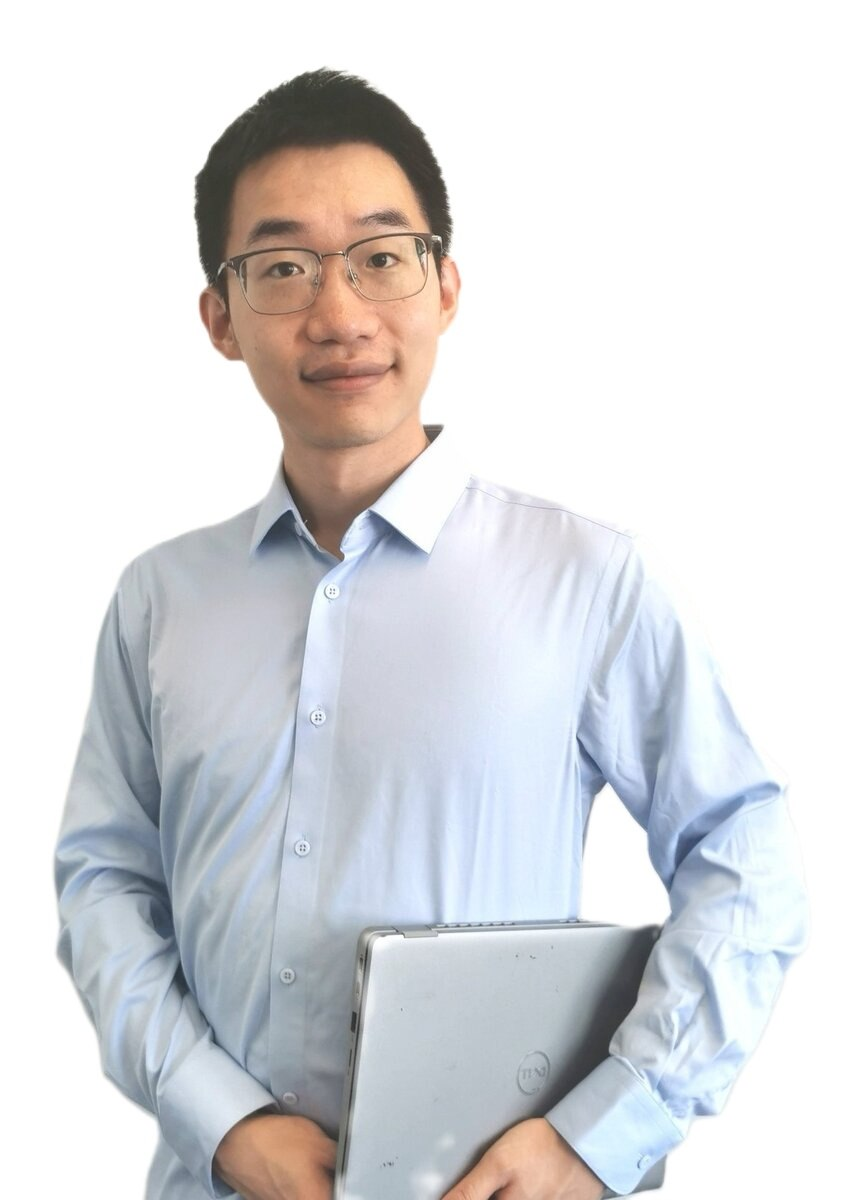
\includegraphics[
            width=0.55\textwidth,
            height=0.45\textheight,
            keepaspectratio
        ]{../zhongli-wang-profile.jpg}
    }{
        \vspace{0.45\textheight}
    }
\end{center}

\vspace{0.7cm}

% \vspace{3cm}


% Personal details
\begin{center}
\renewcommand{\arraystretch}{1.35}
\begin{tabular}{>{\bfseries}p{4.2cm} p{8.5cm}}


Address: & Astastrasse 22, 33617 Bielefeld, Germany \\

Number: & +49 160 9541 6015 \\

Email: & nkwangzhongli@gmail.com \\
\end{tabular}
\end{center}

\vfill

% \begin{center}
%     \small Last updated: \today
% \end{center}
\newpage
\enlargethispage{4\baselineskip}

\begin{flushright}
Zhongli Wang \\
Astastrasse 22 \\
33617 Bielefeld\\
Germany \\
\end{flushright}

\vspace{0.1cm}

\vspace{0.1cm}

\noindent
UNICEF Office of Innovation \\
Systems \& Services – Insights \& Evidence function \\
Stockholm, Sweden \\

\vspace{0.12cm}

\noindent
\textbf{Application for Innovation Data and Product Consultant}

\vspace{0.1cm}

\noindent Dear UNICEF Hiring Committee,

I have successfully completed my Ph.D. in Economics at Bielefeld University (defense: September 21, 2026) and hold an M.A. in Business and Economics with a minor in Data Science. My doctoral research in computational economics, agent-based modeling, and data-driven analysis, combined with my hands-on experience developing data systems and AI-powered workflows, positions me well to contribute to UNICEF's Office of Innovation. I am particularly drawn to this role because it combines technical execution with product design and systems thinking to solve real-world problems.

My background directly aligns with the core areas of this role:

\begin{itemize}
    \item \textbf{Data systems and products:} I have designed and built end-to-end data pipelines, databases, and analytical workflows for complex economic research. I have experience collecting, cleaning, validating, and integrating heterogeneous data sources into reliable information systems. I have developed dashboards and data products that translate raw data into actionable insights for different audiences, from technical teams to senior decision-makers.
    \item \textbf{Automation and AI:} I have developed agent-based computational models and applied machine learning methods (XGBoost, Random Forest, Neural Networks) to automate analysis and extract insights from large datasets. I have hands-on experience with large language models and agentic workflows, including building systems that integrate LLMs into research pipelines for document processing, classification, and knowledge extraction.
    \item \textbf{User research and product discovery:} Through my doctoral research, I have practiced systems thinking and iterative problem-solving, moving from ambiguous research questions to working solutions. I have gathered evidence to test assumptions, refined approaches based on feedback, and designed solutions that balance technical rigor with practical usability.
    % \item \textbf{User adoption and communication:} I have authored peer-reviewed publications, prepared technical reports, and presented research at international conferences. I have strong writing and presentation skills, with experience translating complex technical and analytical concepts clearly for diverse audiences—essential for helping teams adopt and integrate data solutions.
\end{itemize}

My technical skills include strong proficiency in Python, R, SQL, and experience with data visualization. I am comfortable working in Linux-based environments and have developed reproducible, well-documented analytical workflows. I am fluent in English and have C1-level German proficiency, with strong communication skills across technical and non-technical stakeholders.

I am particularly motivated by UNICEF's mission and the opportunity to apply data and AI to advance innovation that benefits children and communities. I thrive in environments that combine technical problem-solving with human-centered design and systems thinking. The role's emphasis on moving quickly from ideas to minimum viable products, testing, and iterating based on real-world use aligns perfectly with my working style and values.

Thank you for considering my application! 
I would welcome the opportunity to discuss how my background in data systems, AI, product design, and systems thinking could contribute to UNICEF's Office of Innovation and its mission to leverage data and knowledge for innovation.

% \vspace{0.08cm}
\noindent Kind regards, \\
\noindent Zhongli Wang
\noindent\hspace{0.5cm}
\includegraphics[width=2.7cm,keepaspectratio]{../Wang-sig.jpg}

\end{document}
% \vspace{0.1cm}
